\subsection{Screen shots}
\begin{figure}[H]
    \centering
    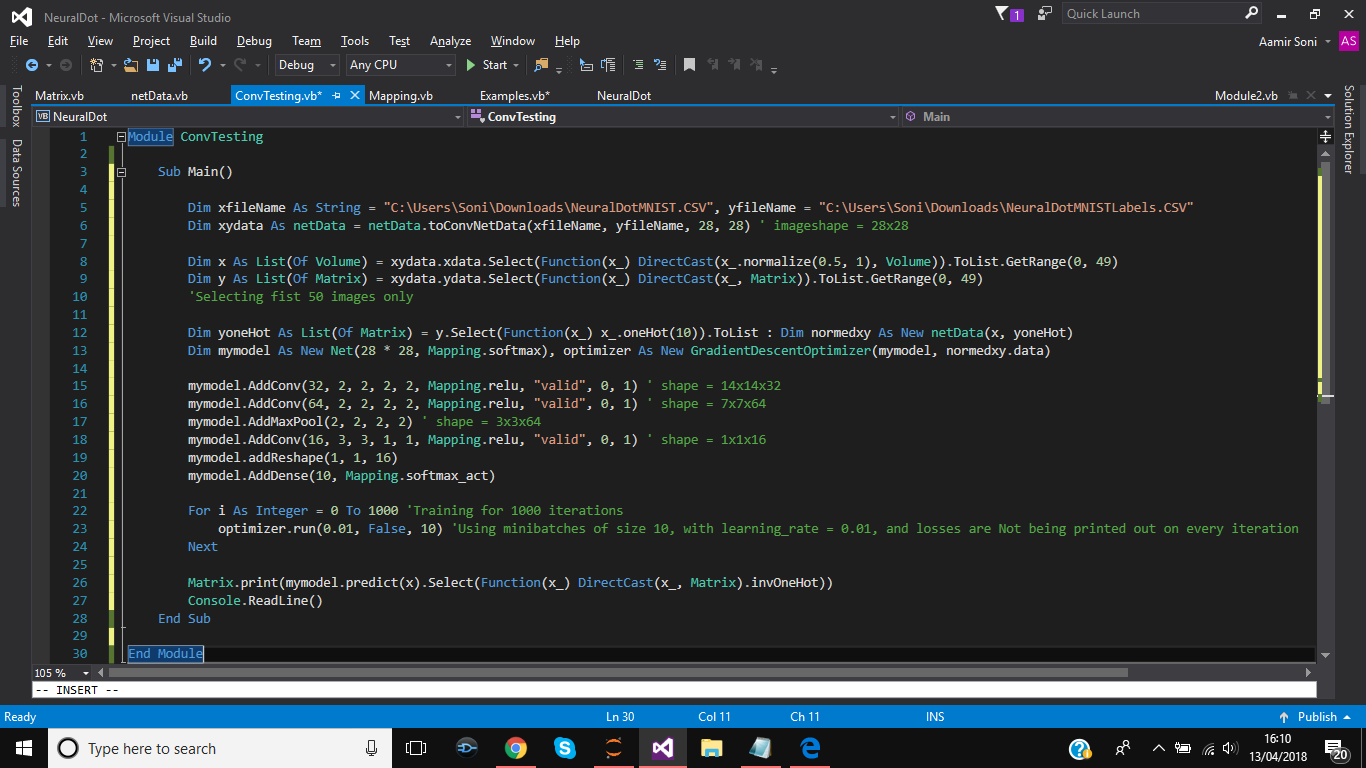
\includegraphics[width=10cm, height=5cm, trim = {0 6.8cm 0 0 }, clip]{Testing/ConvTests/ConvTest1.png}
    \caption{Corresponding code for ConvNet for test 1}
    \label{fig:ConvCodeT1}
    
    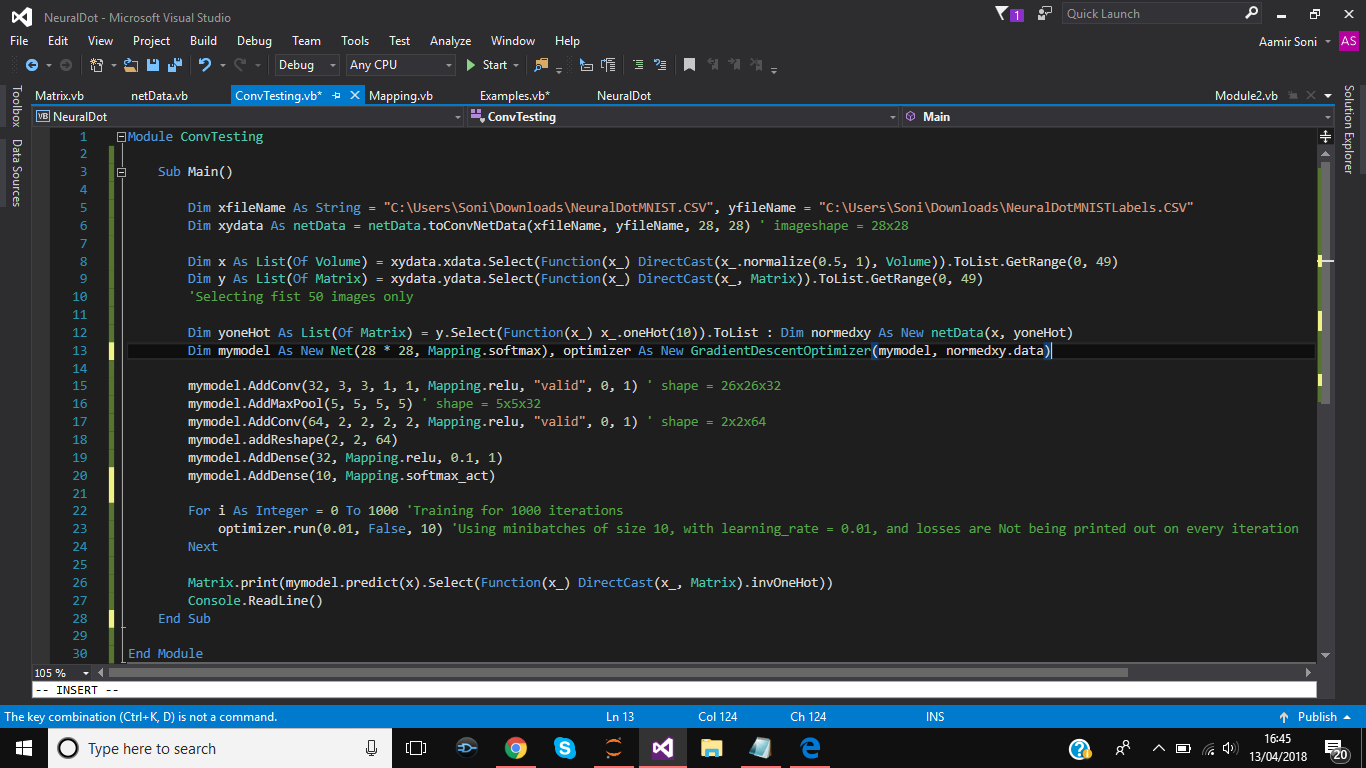
\includegraphics[width=10cm, height=5cm, trim = {0 6.8cm 0 0 }, clip]{Testing/ConvTests/ConvTest2.png}
    \caption{Corresponding code for ConvNet for test 2}
    \label{fig:ConvCodeT2}
    
    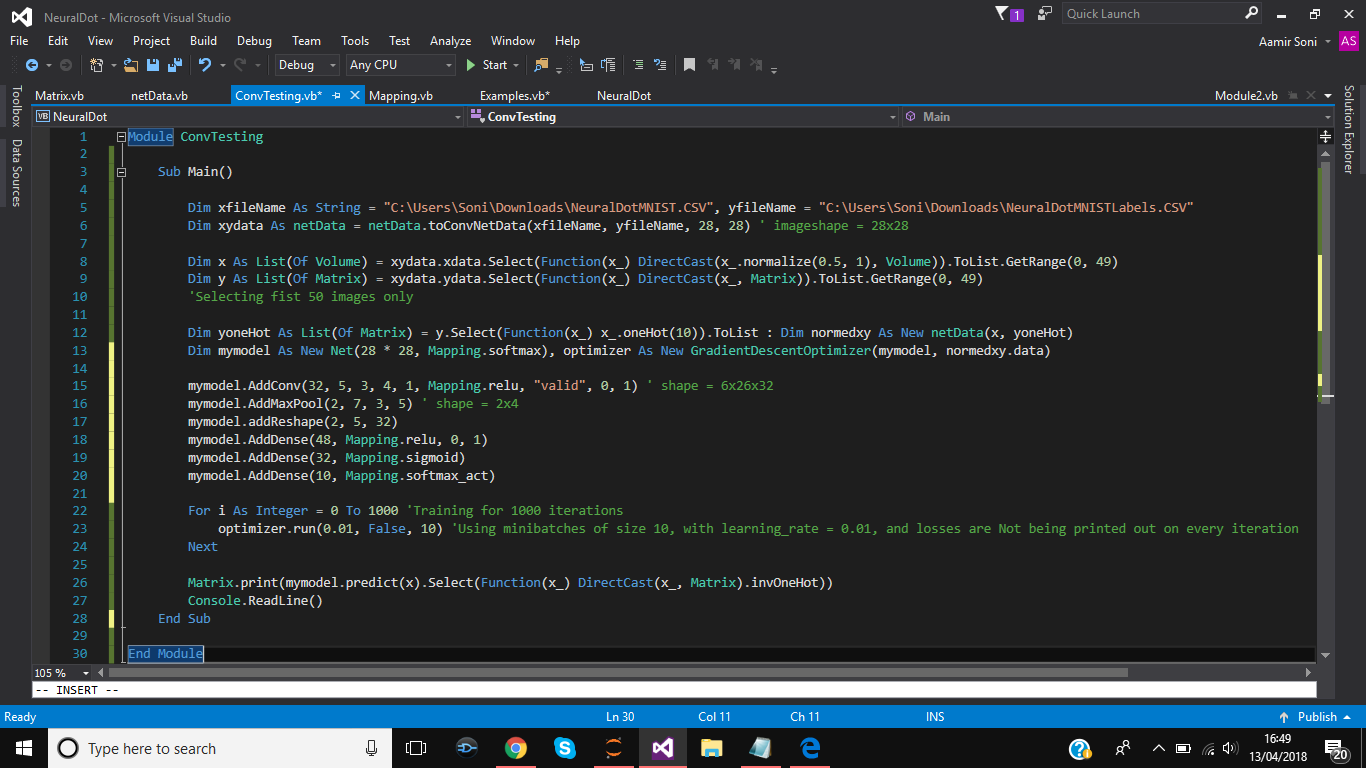
\includegraphics[width=10cm, height=5cm, trim = {0 6.8cm 0 0 }, clip]{Testing/ConvTests/ConvTest3.png}
    \caption{Corresponding code for ConvNet for test 3}
    \label{fig:ConvCodeT3}
\end{figure}

\begin{figure}[H]
    \centering
    
    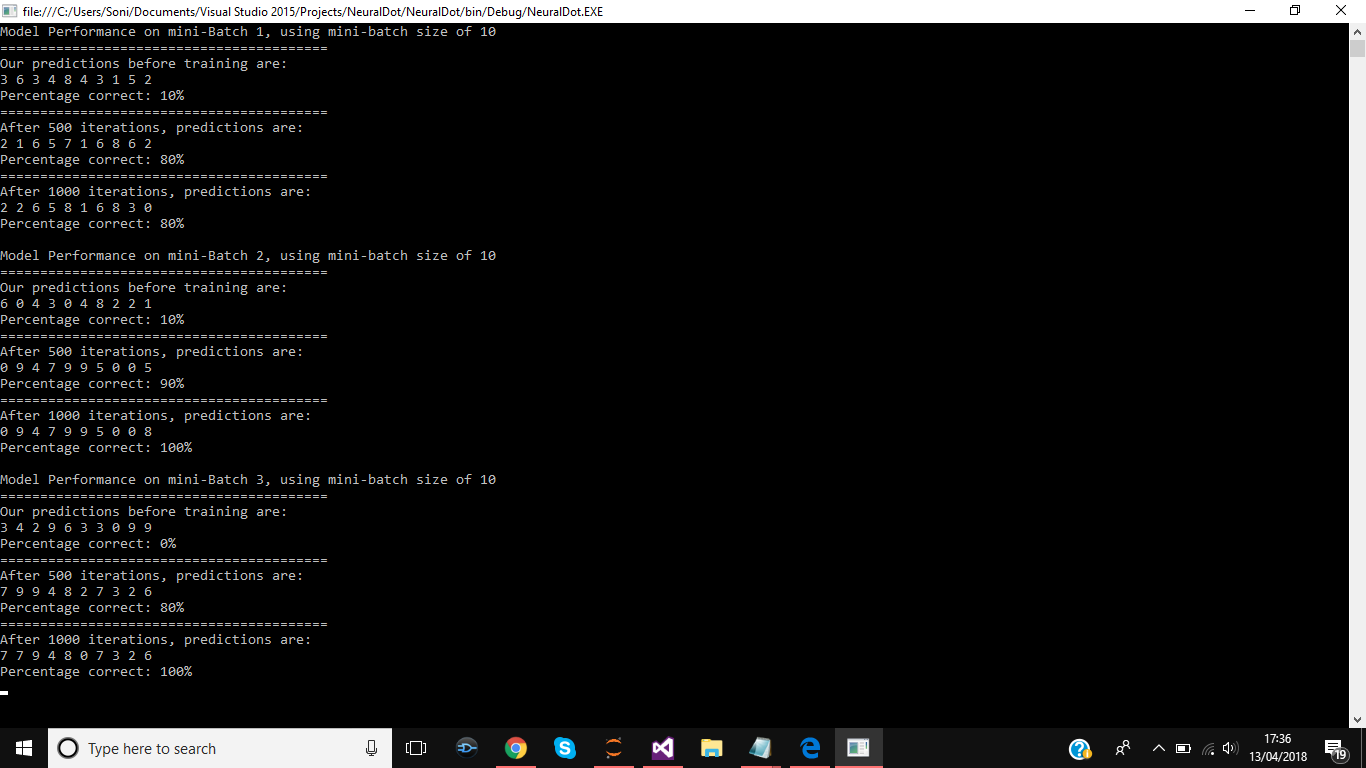
\includegraphics[width=10cm, height=5cm]{Testing/MiniBatchResults/MiniBatchResults1-Test1.png}
    \caption{Results of first model(out of the 200) for Test No1 on Test Set: part 1}
    \label{fig:TestNo1ResultsP1}
    
    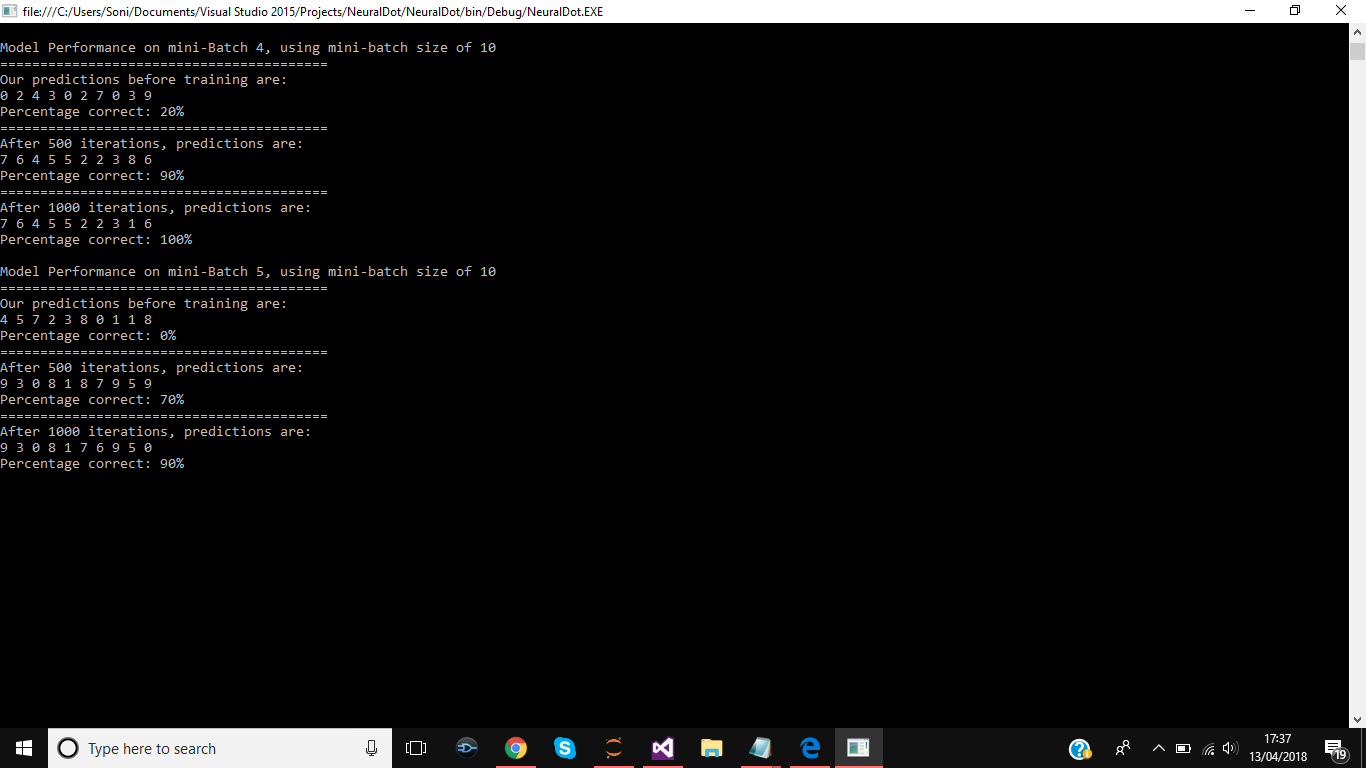
\includegraphics[width=10cm, height=5cm]{Testing/MiniBatchResults/MiniBatchResults2-Test1.png}
    \caption{Results of first model for Test No1 on Test Set: part 2}
    \label{fig:TestNo1ResultsP2}
    
    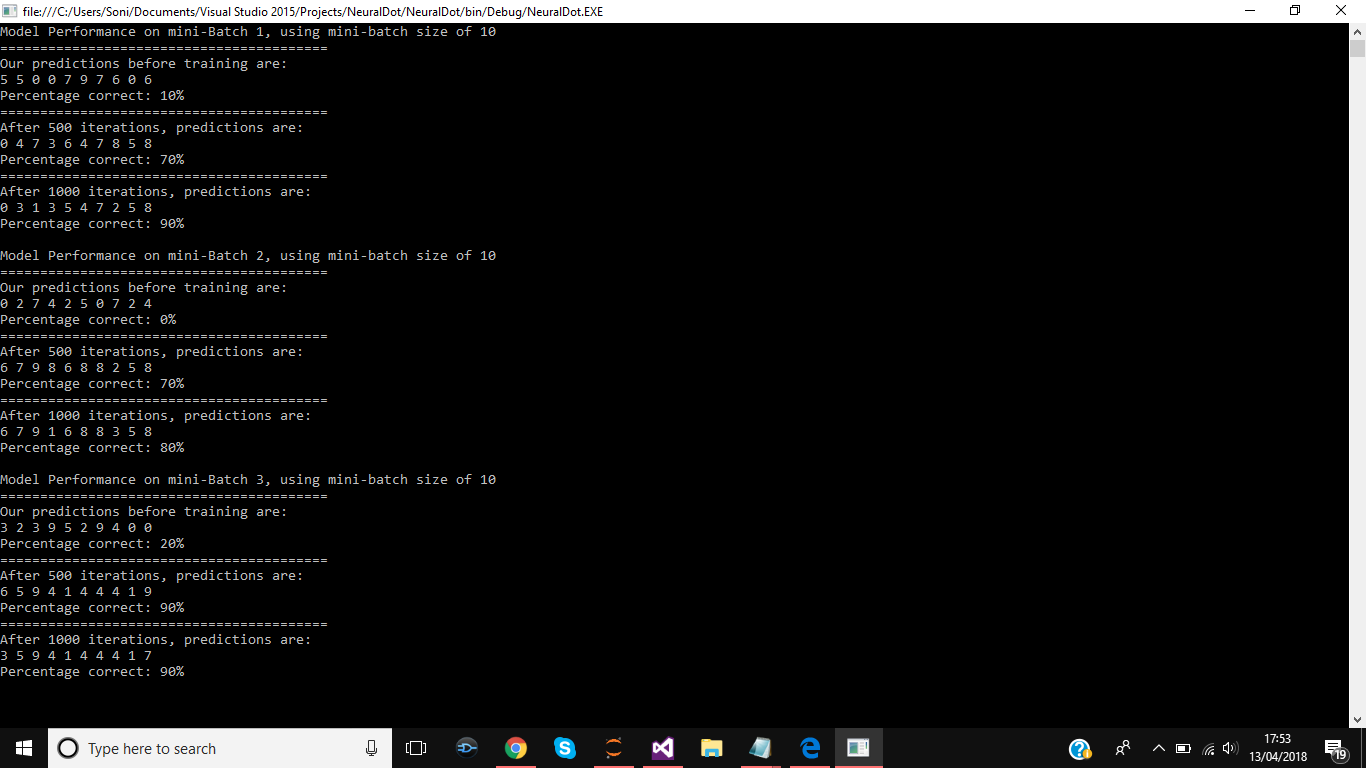
\includegraphics[width=10cm, height=5cm]{Testing/MiniBatchResults/MiniBatchResults1-Test2.png}
    \caption{Results of first model for Test No2 on Test Set: part 1}
    \label{fig:TestNo2ResultsP1}
    
    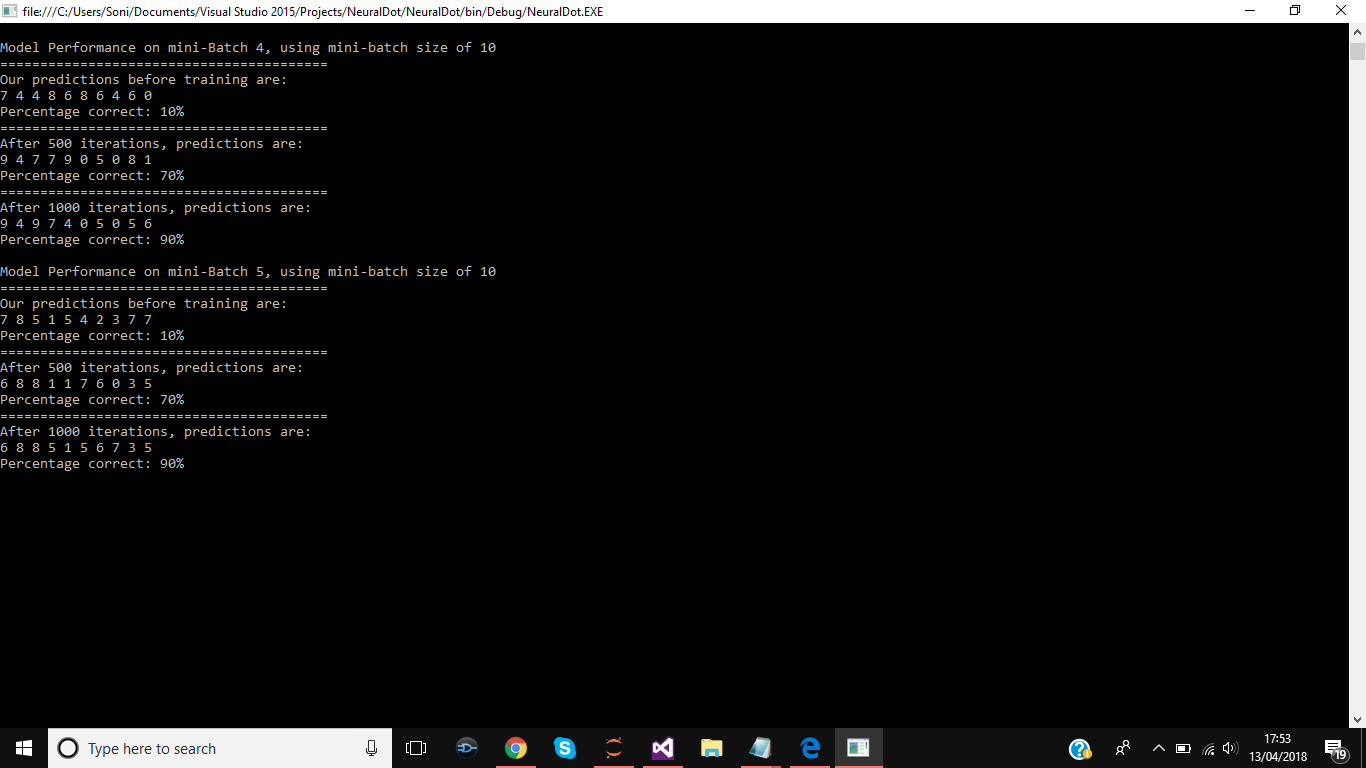
\includegraphics[width=10cm, height=5cm]{Testing/MiniBatchResults/MiniBatchResults2-Test2.png}
    \caption{Results of first model for Test No2 on Test Set: part 2}
    \label{fig:TestNo2ResultsP2}
    
\end{figure}

\newpage

\begin{figure}[H]
    \centering

    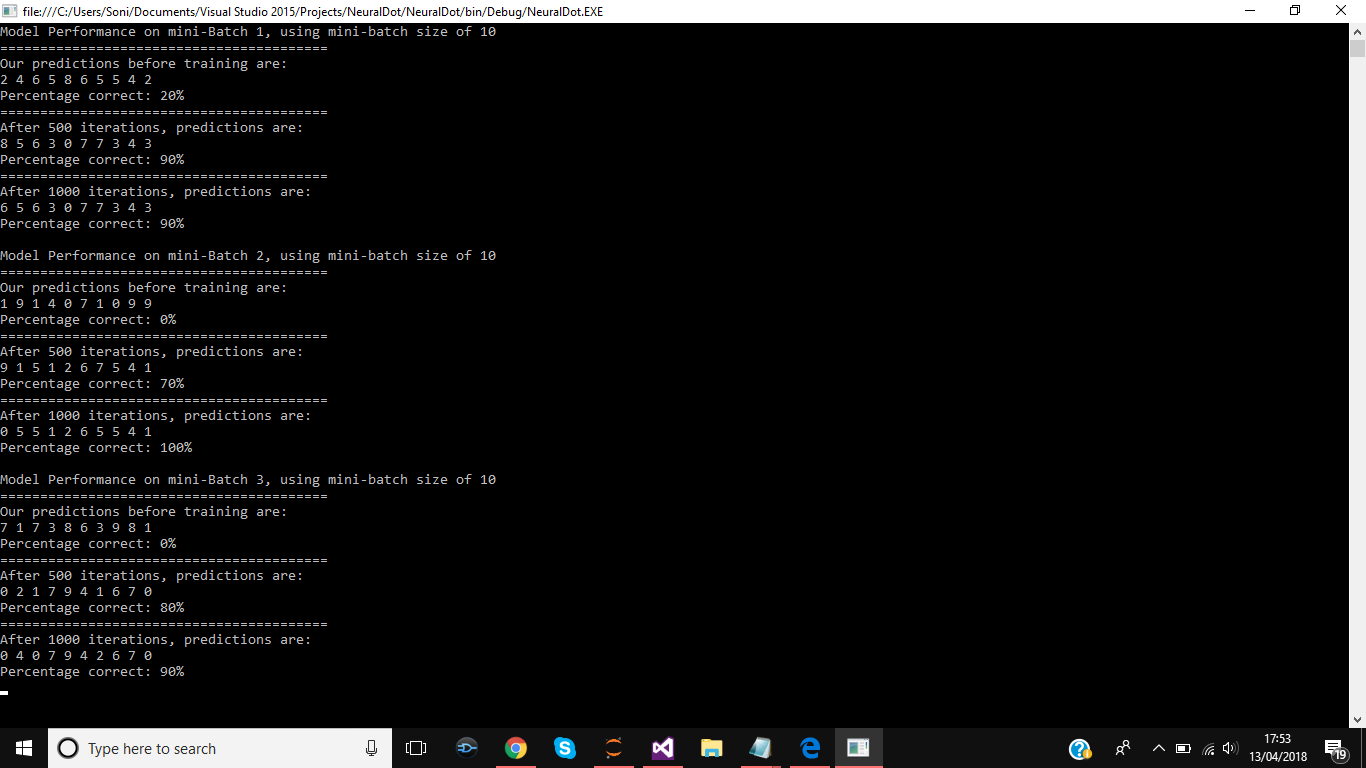
\includegraphics[width=10cm, height=5cm]{Testing/MiniBatchResults/MiniBatchResults1-Test3.png}
    \caption{Results of first model for Test No3 on Test Set: part 1}
    \label{fig:TestNo3ResultsP1}
    
    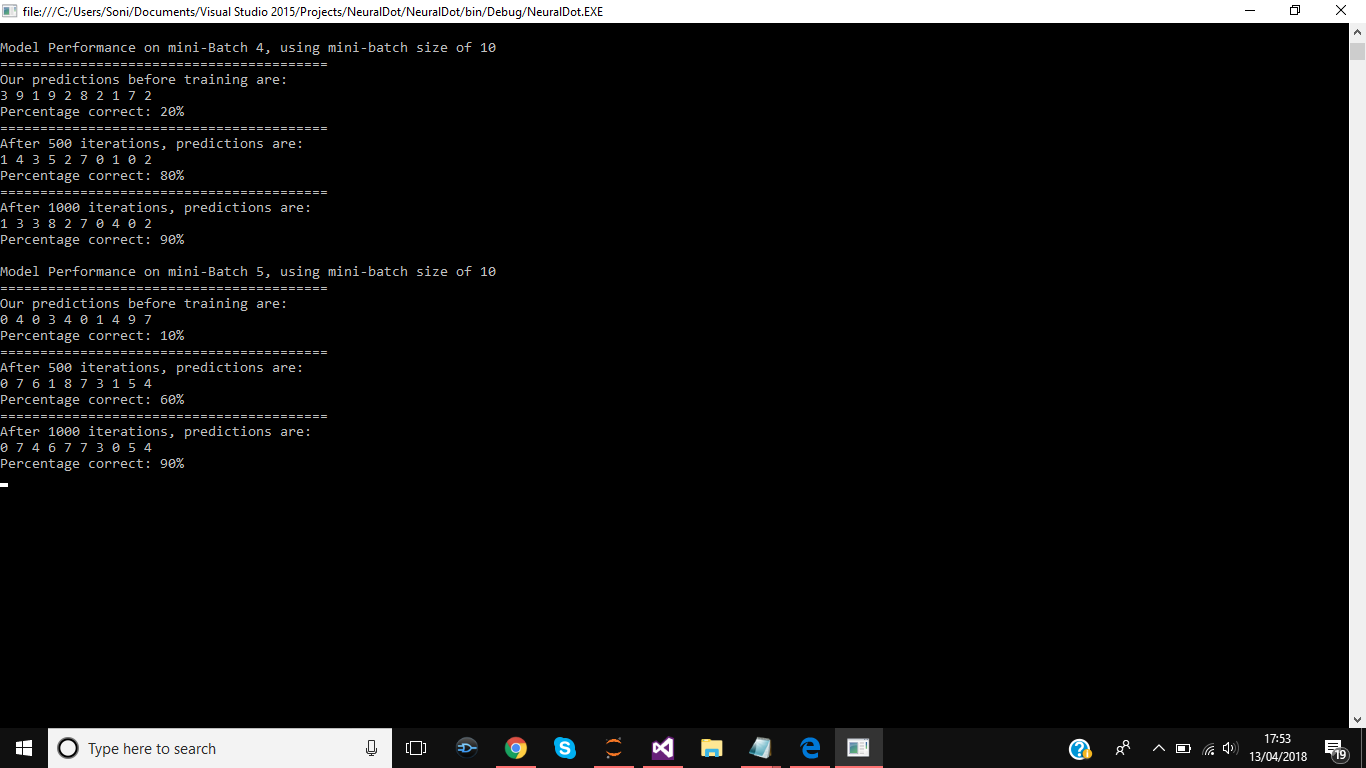
\includegraphics[width=10cm, height=5cm]{Testing/MiniBatchResults/MiniBatchResults2-Test3.png}
    \caption{Results of first model for Test No3 on Test Set: part 2}
    \label{fig:TestNo3ResultsP2}
    
\end{figure}

Below are the YouTube link for the videos for the matrices, volume, and Dense networks tests. A video could not be provided for the convolutional neural networks tests as training conv nets took more than 19 hours in total, hence the reason why the screen shots were provided instead.
\\ \\
I will not be able to record the tests for the dense layer as training each different architecture 100 times on different functions for the sake of reliability takes a long time - as it took approximately 8 hours in total. However, I can record a dense net learning a function instead and training it using a variety of different optimises. 
\\ \\
The playlist below shows an example of this: 
\\
https://www.youtube.com/watch?v=8UlRKepX28g\&list=PLfRtphbl3o-0VLaZzFeRyGXw8GK2RV5T7
\\ \\
In the playlist above, we used a dense net to learn a function. We then made the function (data), much more difficult and we see that the ADAM optimiser is able to train the net to learn the function to a good degree of accuracy while the RMS optimiser is not able to do this.
\\ \\
Finally, the link for the testing of some of the functions of the matrix and Volume classes are below:
\\ \\
Matrix Testing video: https://www.youtube.com/watch?v=M1PnV63fa2g
\\
Volume Testing video: https://www.youtube.com/watch?v=aO6wxGt3G58
\\ \\
Note: Not every function was tested in the video, however in the testing section every function was tested thoroughly.
